%% Springer Nature LaTeX template (sn-jnl) build for submission to
%% Nonlinear Dynamics (Springer). Two-system manuscript: the mean-field
%% (two-population Sakaguchi--Kuramoto) study plus the nonlocal-ring chimera
%% collapse study, with the critical-review (C1/C2) validations folded into the
%% main text. Reference style: sn-mathphys (Math & Physical Sciences, Numbered).
%% Swap to [pdflatex,sn-basic,Numbered] if the journal's submission page
%% specifies the Basic style instead; both .bst files are shipped.
%%
%% Compatibility: the shipped sn-jnl.cls (v0.1, 2019) uses manyfoot's footnote
%% machinery (\SetFootnoteHook, \DeclareNewFootnote) and xcolor's \definecolor
%% in its begin-document hook without loading either package; preload them so
%% the document compiles on current TeX distributions.
\RequirePackage{manyfoot}
\RequirePackage{xcolor}
\documentclass[pdflatex,sn-mathphys,Numbered]{sn-jnl}

\usepackage{graphicx}%
\usepackage{amsmath,amssymb,amsfonts}%
\usepackage{booktabs}%
\usepackage[title]{appendix}%
\graphicspath{{figures/}{paper_figures/}{paper/critical_review_figs/}}

%% sn-jnl's \orcid macro renders an ORCID logo image (Orcidlogo.eps) that is not
%% part of this build; redefine it to typeset the iD as linked text so the
%% document is self-contained and compiles without the logo file.
\makeatletter
\gdef\orcid#1{\href{https://orcid.org/#1}{\footnotesize\,(ORCID: #1)}}
\makeatother

\begin{document}

\title[Chimera Collapse Ages]{Chimera Collapse Ages: Topology-Dependent Finite-Size Scaling in Mean-Field and Ring Oscillator Systems}

\author*[1]{\fnm{Avery} \sur{Karlin}\orcid{0000-0003-3848-6782}}\email{averykarlin3@gmail.com}

\affil*[1]{\orgname{Independent Researcher}}

\abstract{We report a long-duration empirical study of chimera collapse in two canonical
settings: the two-population Sakaguchi--Kuramoto system with strictly identical
natural frequencies, on the oscillator engine of a deployed additive synthesizer at
small population sizes ($N = 4$--$64$ per population), and the nonlocally coupled
ring near its chimera existence boundary. In the mean-field system, the operational
collapse detector --- and the first-passage criterion standard for chimera
lifetimes --- measure the wrong observable: up to 98\% of sustained near-synchrony
crossings recover as the chimera re-forms, and 69--97\% of detector firings are
self-healing \emph{grazes}. Under an absorption-grade label, true lifetimes at the
operating corner ($A = 0.5$, $\beta = 0.05$) double, become $N$-independent
($\tau_{\mathrm{abs}} \approx 139$\,s over a $16\times$ range of $N$), and age
(Weibull shape $2.3$--$3.0$, surviving stratification on the collective initial
condition). Deaths are breath-synchronized and ratchet: per-cycle envelope maxima
grow monotonically to capture. The reduced two-population model of Abrams
\emph{et al.}, validated against its published bifurcations with no fitted
parameters, explains the inversion --- the operating corner lies beyond the
homoclinic, so the deployed ``chimera'' is a transient spiraling out along a
destroyed limit cycle's ghost, while the nominally unreliable corner ($A = 0.2$)
holds the only true attractor --- yet captures $3.2\times$ faster than the
finite-$N$ system dies; a direct test rules out additive collective noise, leaving
that prolongation mechanism open. On the ring ($\beta = 0.110$--$0.130$,
$N = 32$--$256$, $7{,}500$ pre-registered runs), collapse is again an aging
process: the Weibull shape exceeds one in every $(\beta, N)$ cell and rises with
$N$ before saturating to a finite $k_\infty \approx 1.35$--$1.65 > 1$ (bootstrap
intervals excluding one) that grows toward criticality. The dying object is a
genuine chimera in $97$--$98\%$ of runs and the result is robust to the death
criterion --- but median ring lifetimes \emph{decrease} with $N$ on the
near-boundary side, opposite to the mean-field plateau. The aging of chimera
collapse is topology-independent; its finite-size scaling is topology-dependent.}

\keywords{chimera states, coupled phase oscillators, Kuramoto--Sakaguchi model, nonlocal coupling, finite-size scaling, transient dynamics, Weibull aging hazard}

\maketitle

\begin{quote}\itshape
Chimera states, in which a population of identical oscillators
spontaneously splits into one synchronized group and one disordered group, are
usually studied as a question in pure mathematics. Here the same phenomenon appears
inside a working music synthesizer, where two coupled oscillator banks shape the
sound and the software periodically judges the pattern ``dead'' and restarts it.
Asking why it dies so often reveals that the restart trigger was watching the wrong
quantity: most apparent deaths are momentary lapses that heal on their own. Once the
genuine deaths are isolated, they prove regular, rhythmic, and no more frequent in
large populations than small ones --- and a simple reduced model explains where and
why they occur, while underpredicting how long the pattern survives, a discrepancy
the paper leaves as an open problem. A second, classical test bed --- a ring of
oscillators coupled to their near neighbors --- shows the same aging of collapse
risk but the opposite dependence on population size, separating what is universal
about chimera death from what belongs to the network's shape.
\end{quote}

\section{Introduction}\label{sec:intro}

Chimera states --- the coexistence of synchronized and desynchronized populations in
systems of identical coupled oscillators --- have been a central object of nonlinear
dynamics since their discovery by Kuramoto and Battogtokh~\cite{kb2002} and naming by
Abrams and Strogatz~\cite{as2004}. The two-population model of Abrams, Mirollo,
Strogatz, and Wiley~\cite{abrams2008} made the phenomenon solvable: two identical
populations with stronger intra- than inter-population coupling support stable
chimeras, breathing chimeras born in a Hopf bifurcation, and a homoclinic boundary
beyond which no chimera attractor survives. At finite size the picture is enriched by
transience: on nonlocally coupled rings, chimeras are chaotic transients whose
lifetimes grow with oscillator count~\cite{wo2011}, and the finite-$N$ fate of
chimeras has remained a recurring theme of the literature
since~\cite{pa2015,om2018}, including for two small populations of the kind
studied here~\cite{panaggio2016}.

This paper studies chimera collapse in an unusual arena: the oscillator engine of a
deployed real-time additive synthesizer, in which a two-population
Sakaguchi--Kuramoto bank with \emph{strictly identical} natural frequencies drives
the partial amplitudes of a musical voice, and a supervisor process re-seeds the
chimera whenever an engineering detector declares it dead. Coupled-oscillator
networks have an established history as sound-synthesis drivers~\cite{lem2019,lemsmc};
here the synthesis application matters to the dynamics only in that it fixes the
regime of interest --- small populations ($N = 4$--$64$ per side), long unattended
runtimes, and a specific operating corner chosen, as it turns out, for the wrong
reason. The deployment prompts a question the theory literature rarely needs to ask
operationally: \emph{what exactly is the death of a chimera, and what does a detector
of it actually detect?}

The deployment fixes only the mean-field half of a larger question: which features
of chimera collapse are universal, and which are properties of the coupling
topology? The two-population mean field and the nonlocally coupled ring are the two
canonical chimera substrates, and they make opposite finite-size predictions in
their classic regimes --- ring chimera lifetimes grow with oscillator
count~\cite{wo2011}, while Sec.~\ref{sec:stats} shows the mean-field lifetimes are
flat in $N$. We therefore close the paper by carrying the same survival methodology
to the ring near its existence boundary (Sec.~\ref{sec:ring}), where lifetimes are
finite at feasible compute, asking whether the aging structure of collapse --- the
rising hazard --- transfers across topology even where the lifetime scaling does
not.

We answer with a chain of measurements, each gating the next, on bit-reproducible
integrators (2{,}100 baseline mean-field runs plus targeted re-campaigns, and
7{,}500 pre-registered ring runs; every figure regenerable from committed
configurations). The contributions are:

\begin{enumerate}
\item \textbf{Graze versus absorption.} The operational collapse criterion ---
sustained near-synchrony of the incoherent population --- overwhelmingly fires on
events the chimera survives: up to 98\% of criterion-satisfying crossings recover,
and 69--97\% of the deployed detector's firings are such grazes. We introduce a
two-timescale, absorption-grade labeling and show first-passage ``lifetimes'' are
roughly half the true absorption times (Sec.~\ref{sec:graze}).
\item \textbf{An inverted stability picture.} Under absorption labeling, lifetimes at
the operating corner are $N$-independent ($\approx 139$\,s, $N = 4$--$64$, every seed
absorbing), while at the nominally unreliable high-morph corner the majority of seeds
\emph{never} absorb: the operating corner has no chimera attractor at all, and the
discarded corner holds the only persistent chimera in the system
(Sec.~\ref{sec:stats}).
\item \textbf{The death mechanism.} Collapse is a breath-synchronized ratchet:
collapse attempts and true deaths lock to a phase of the breathing cycle, successive
per-cycle envelope maxima grow monotonically (spiraling out exponentially toward the
synchronization boundary), and hazard rises with cycle index. Transverse escape from
the Poisson submanifold is ruled out by a validated observable and a null
interventional test; lifetime is instead organized by the collective initial
condition, dominantly the inter-population phase offset (Sec.~\ref{sec:mechanism}).
\item \textbf{Closure by the reduced model --- and a clean open problem.} The reduced
equations of Ref.~\cite{abrams2008}, validated against that paper's own published
results and applied with a literal 1:1 timescale and zero fitted parameters, place
the operating corner beyond the homoclinic ($A_{hc}(\beta{=}0.05) = 0.4096$),
reproduce the breath period and per-cycle spiral rates, identify the never-absorbers'
level with the stable chimera's $r^*$, and predict individual run lifetimes beyond
any static feature of the seed. They also fail in one instructive way: mean-field
capture is $3.2\times$ faster than finite-$N$ death, and the flat
$\tau_{\mathrm{abs}}(N)$ is absent from the $N$-free collective flow --- finite-size
fluctuations \emph{extend} the transient (Sec.~\ref{sec:reduced},
Sec.~\ref{sec:discussion}).
\item \textbf{Topology comparison: aging transfers, scaling does not.} On the
nonlocally coupled ring near its existence boundary, collapse is also an aging
process: the censored-Weibull shape exceeds one, with confidence intervals
excluding one, in all 15 pre-registered $(\beta, N)$ cells, and rises with $N$
before saturating to a finite $k_\infty \approx 1.35$--$1.65 > 1$ that grows toward
criticality (Appendix~\ref{app:ring}). The dying object is validated as a genuine
chimera in $97$--$98\%$ of runs and the hazard shape is robust to the death
criterion. Median ring lifetime, however, \emph{decreases} with $N$ in this regime
--- opposite to both the deep-stable ring growth~\cite{wo2011} and the mean-field
plateau: the aging of chimera collapse is topology-independent, while its
finite-size scaling is topology-dependent (Sec.~\ref{sec:ring}).
\end{enumerate}

\section{Systems}\label{sec:system}

\subsection{The two-population mean-field system}\label{sec:system:meanfield}

The voice integrates two populations $\sigma \in \{1, 2\}$ of $N$ phase oscillators
each,
\begin{equation}
\dot\theta_i^\sigma \;=\; \omega \;+\; \sum_{\sigma'} \frac{K_{\sigma\sigma'}}{N}
\sum_{j=1}^{N} \sin\!\big(\theta_j^{\sigma'} - \theta_i^{\sigma} - \alpha\big),
\label{eq:model}
\end{equation}
with intra-population coupling $K_{\sigma\sigma} = \mu = (1+A)/2$, inter-population
coupling $K_{\sigma\sigma'} = \nu = (1-A)/2$ ($\mu + \nu = 1$, $A = \mu - \nu$), and
phase lag $\beta = \pi/2 - \alpha$~\cite{kuramoto1984,sk1986}, matching the
conventions of Ref.~\cite{abrams2008}. A code audit confirms the natural frequencies are identical
\emph{exactly} ($\delta\omega = 0$: no per-oscillator frequency term, detuning
explicitly zeroed on this path), so the dynamics is deterministic given the initial
condition and collapse cannot be attributed to frequency disorder; we work in the
$\omega = 0$ rotating frame. Integration is fourth-order Runge--Kutta with
$dt = 0.05$ at a documented one-model-unit-per-second clock, so all times below are
seconds with no conversion; halving and quartering $dt$ leaves lifetime
distributions statistically indistinguishable (two-sample KS $p = 1.0$). All runs are
bit-reproducible from logged (seed, parameters, $dt$); every re-analysis below begins
by reproducing the upstream labels exactly.

In the application, the incoherent population's per-oscillator coherences modulate
the gains of an additive partial bank, $g_i' = g_i\,[\,1 + d\,a\,(c_i - \tfrac12)\,]$
with $c_i = \tfrac12(1 + \cos(\theta_i - \psi))$, turning the chimera's collective
dynamics into a slowly self-morphing spectrum; the synthesis layer plays no further
role in the dynamics studied here. Runs are initialized with the canonical chimera
seed (one population tightly clustered, the other spread), since spontaneous chimera
formation from random phases is negligible in this regime. The deployed supervisor
declares the state alive while $\max_\sigma R_\sigma > 0.9$ and
$\min_\sigma R_\sigma < 0.85$, fires after 2\,s of sustained violation, and re-seeds
the incoherent population. The baseline campaign comprises 200 seeds per population
size at the operating corner ($A = 0.5$) and 100 at the high-morph corner
($A = 0.2$), $N \in \{4, 8, 16, 24, 32, 48, 64\}$, $\beta = 0.05$ throughout,
integrated unsupervised to $t_{\max} = 2000$\,s.

\subsection{The nonlocally coupled ring}\label{sec:system:ring}

The second system is the canonical substrate of chimera-death studies, the
nonlocally coupled ring~\cite{kb2002,wo2011}: $N$ phase oscillators with top-hat
coupling to their $P$ nearest neighbors on each side,
\begin{equation}
\dot\theta_k \;=\; -\frac{1}{2P+1} \sum_{|j-k|\le P}
\sin\!\big(\theta_k - \theta_j + \alpha\big),
\qquad P = \mathrm{round}(rN),
\label{eq:ring}
\end{equation}
with coupling radius $r = 0.15$, phase lag $\alpha = \pi/2 - \beta$, identical
frequencies in the rotating frame, and the same fixed-step RK4 integration scheme
(validated against an independent reference implementation). The natural order
parameter is local: $\rho_k = |(2P+1)^{-1} \sum_{|j-k| \le P} e^{i\theta_j}|$, the
modulus of the windowed mean field, whose spatial profile separates a chimera's
coherent arc ($\rho_k \approx 1$) from its incoherent arc (low $\rho_k$). Death of
the ring chimera is the loss of this spatial structure: the event criterion is the
spatial standard deviation $\rho_{\mathrm{std}}(t)$ of the $\rho_k$ field falling
below $\varepsilon_{\mathrm{std}} = 0.04$ and staying below for $50$ time units,
with right-censoring at $T_{\max} = 12{,}000$; Sec.~\ref{sec:ring} validates this
criterion against alternatives and against the identity of the dying object. The
ring campaign --- design, event definition, primary endpoint (the censored-Weibull
shape $k$ with profile-likelihood intervals), and decision rule all pre-registered
before any production run --- comprises
$\beta \in \{0.110, 0.115, 0.120, 0.125, 0.130\}$ approaching the existence
boundary --- $\beta_c = 0.137$ [$0.130, 0.144$], measured independently in
Appendix~\ref{app:betac} and consistent with the literature range
$\beta_c \approx 0.13$--$0.14$ --- at $N \in \{32, 64, 128\}$ with $300$ runs
per cell ($4{,}500$ runs), later extended at all five $\beta$ to $N = 192$ and
$256$ ($3{,}000$ further runs) for the thermodynamic-limit extrapolation of
Appendix~\ref{app:ring}.

\section{Graze versus absorption}\label{sec:graze}

What counts as the death of a chimera? In a deployed system the answer is
operational: the supervisor's aliveness condition fails continuously for 2\,s, and
our initial lifetime campaign used the closely related first-passage criterion that
$\min(R_1, R_2)$ exceed a threshold $\theta = 0.85$ sustained for $W = 5$\,s. Both
definitions encode the same assumption: that a sustained excursion of the incoherent
population to near-synchrony \emph{is} the death of the chimera. This section shows
that assumption is wrong, and replaces it.

\subsection{Threshold crossings overwhelmingly recover}

Extending the recorded trajectories past their first criterion-satisfying crossing,
rather than terminating there, reveals that the crossing is usually not absorbing. At
the operating corner and across $N = 8$--$64$, up to 98\% of first crossings ---
excursions exceeding $\theta$ for longer than the full 5\,s sustain window --- are
followed by recovery: the incoherent population desynchronizes again, with
post-crossing minima of $\min(R_1, R_2)$ clustering at 0.2--0.45, a fully re-formed
chimera. About two-thirds of these recovered trajectories are later absorbed for
good; the remainder churn through further graze--recover cycles. The first sustained
crossing is therefore a \emph{graze} of the synchronization boundary, not a death,
and first-passage lifetimes computed from it measure time-to-first-long-graze.

Figure~\ref{fig:trace} shows a representative trajectory ($N = 16$, $A = 0.5$; seed
pinned in the released configuration). The run grazes twice --- each time exceeding
$\theta$ for more than 5\,s before the chimera re-forms --- and is absorbed on its
third approach at $t_{\mathrm{abs}} = 221.9$\,s, having first ``collapsed'' by the
engineering criterion at $t_{\mathrm{graze}} = 83.2$\,s. The shipped supervisor's
detector fires \emph{six times} on this trajectory before the single event that is
irreversible: six firings, two reforms, one death.

\begin{figure}[t]
\centering
\includegraphics[width=0.95\linewidth]{fig1}
\caption{A graze is not a death. $\min(R_1, R_2)$ for a single run ($N = 16$,
$A = 0.5$, $\beta = 0.05$; breath period $T_b = 20.5$\,s). The trajectory crosses
$\theta = 0.85$ (upper line) in sustained excursions twice, recovering below the
0.80 recovery threshold (lower line) each time as the chimera re-forms, before the
absorbing crossing at $t_{\mathrm{abs}} = 221.9$\,s. The engineering first-passage
label $t_{\mathrm{graze}} = 83.2$\,s and the six firings of the deployed 2-s detector
are marked.}
\label{fig:trace}
\end{figure}

\subsection{An absorption-grade label}

We therefore assign every run two timescales from a single trace. The first,
$t_{\mathrm{graze}}$, is the unmodified first-passage label, retained for
comparability. The second, $t_{\mathrm{abs}}$, is the time of the first crossing
\emph{not} followed by recovery --- $\min(R_1, R_2) < 0.80$ sustained at least
5\,s --- within a verification horizon $T_v = 120$\,s; runs still alternating
between grazes and recoveries at the integration horizon are right-censored.

The absorption label is robust to its own knobs where it matters. Sweeping
$T_v \in \{60, 120, 240\}$\,s against recovery thresholds $\{0.75, 0.80\}$ moves
$\hat\tau_{\mathrm{abs}}$ by 22--27\% at $A = 0.5$, monotonically in $T_v$ and
negligibly in the recovery threshold --- comparable to or better than the
$\sim$52\% $(\theta, W)$-sensitivity of the graze criterion itself. At $A = 0.2$
the apparent sensitivity is dominated by censoring rather than the labeling
parameters, for a reason Sec.~\ref{sec:stats} shows is dynamical: most $A = 0.2$
trajectories never absorb at all.

The quantitative consequence at the operating corner is a factor of two:
$\hat\tau_{\mathrm{graze}} \approx 63$--$67$\,s against
$\hat\tau_{\mathrm{abs}} \approx 139$\,s (Fig.~\ref{fig:tau}). First-passage chimera
lifetimes computed with engineering-style criteria systematically measure the wrong,
and roughly halved, quantity.

\subsection{The deployed detector is a graze detector}

Replaying the shipped detector over the same unsupervised trajectories and
classifying each firing by whether the underlying event self-recovers gives
Table~\ref{tab:overtrigger}: 69--79\% of firings at $A = 0.5$, and 95--97\% at
$A = 0.2$, occur on grazes the chimera survives on its own. The deployed system has
been re-seeding a state that was mostly not dead --- harmless in practice, since
re-seeding lands near where the trajectory already was, but diagnostic of the
conceptual gap this section closes: engineering collapse detection and dynamical
absorption are different observables. All statistics below are computed on
$t_{\mathrm{abs}}$ unless noted.

\begin{table}[t]
\centering
\caption{Supervisor over-trigger: fraction of the deployed 2-s detector's firings,
replayed over unsupervised traces, occurring on self-recovering grazes.}
\label{tab:overtrigger}
\begin{tabular}{ccccc}
\toprule
$A$ & $N$ & firings/run & over-trigger & median wasted (s) \\
\midrule
0.5 & 8  & 7.2  & 79\% & 4.4 \\
0.5 & 16 & 5.2  & 76\% & 2.4 \\
0.5 & 32 & 4.1  & 73\% & 3.9 \\
0.5 & 64 & 3.3  & 69\% & 5.3 \\
0.2 & 8  & 12.3 & 95\% & 2.0 \\
0.2 & 16 & 9.8  & 97\% & 1.8 \\
0.2 & 32 & 7.9  & 96\% & 1.7 \\
0.2 & 64 & 4.7  & 95\% & 1.8 \\
\bottomrule
\end{tabular}
\end{table}

\begin{figure}[t]
\centering
\includegraphics[width=0.85\linewidth]{fig2}
\caption{Graze versus absorption lifetimes. Exponential-MLE
$\hat\tau_{\mathrm{graze}}$ and $\hat\tau_{\mathrm{abs}}$ versus $N$ at both
coupling disparities. At $A = 0.5$ absorption lifetimes are $\approx 2.2\times$ the
first-passage values and flat in $N$; at $A = 0.2$ no absorption lifetime is
defined for the majority of seeds (Sec.~\ref{sec:stats}).}
\label{fig:tau}
\end{figure}

\section{Absorption statistics at finite $N$}\label{sec:stats}

\subsection{A flat plateau at the operating corner}

At $A = 0.5$, every one of the 1{,}400 seeds absorbs within the horizon (0\%
censored at every $N$), and the absorption lifetime is $N$-independent:
$\hat\tau_{\mathrm{abs}} = 139, 152, 143, 131, 136, 136, 135$\,s for
$N = 4$--$64$, a ratio $\tau(64)/\tau(4) = 0.97$ over a sixteen-fold range of
population size, with fitted exponential rate in $N$ indistinguishable from zero.
The weak rise from $N = 4$ to $16$ visible in the graze times
($39 \to 72$\,s) does not survive absorption labeling --- it was a graze artifact.
The published-style picture of a lifetime that grows with oscillator count, familiar
from ring-topology chimeras~\cite{wo2011}, is absent here in both label and shape:
adding partials does not buy persistence at this corner, at any tested $N$.

\subsection{The inversion: the high-morph corner does not absorb}

The corner the application had classified as unreliable behaves in the opposite way.
At $A = 0.2$, between 51\% and 78\% of seeds (rising with $N$) \emph{never absorb}:
extending the horizon eightfold to $t_{\max} = 16{,}000$\,s leaves the censored
fraction essentially unchanged, so the censoring is irreducible --- a dynamical
finding, not a horizon artifact. The minority that does absorb does so promptly and
increasingly on the first approach: the zero-graze fraction among absorbers rises
from 0.08 at $N = 4$ to 0.96 at $N = 64$. Capture at $A = 0.2$ is bimodal ---
absorb almost immediately, or settle into a persistent, intermittently grazing
chimera~\cite{sudaokuda2015} with no defined absorption time. The stability assumption of the deployment is
therefore inverted: the ``reliable'' corner always dies, and the ``risky'' corner
contains the only persistent, non-absorbing chimeras in the system. Section~\ref{sec:reduced} shows
both facts are exactly where the bifurcation diagram says they should be.

\subsection{Aging: hazard rises with every breath}

Absorption at $A = 0.5$ is not memoryless. Censored-Weibull fits give shape
parameters $k_{\mathrm{abs}}$ of $2.27$, $2.22$, $2.49$, $2.67$, $2.44$, $2.72$, and
$3.03$ for the seven sizes $N = 4$--$64$, all confidence intervals well above 1 (Fig.~\ref{fig:weibull}) ---
stronger aging than in the graze times ($k_{\mathrm{graze}} = 0.82$--$2.19$), so the
survival shoulder is not a labeling artifact.

Nor is the aging an artifact of pooling heterogeneous deterministic transients
across the seed ensemble. Because the dynamics is deterministic, a fitted $k > 1$
could in principle encode only the \emph{spread of fixed transient times} across
initial conditions rather than a hazard that rises along each trajectory. We
separate the two by stratifying the seed ensemble at each $N$ into four
equal-count bins of a collective initial-condition coordinate --- the
inter-population phase gap $|\Delta\phi_0|$, the initial incoherent-population
level $\overline{R}_{\mathrm{incoh},0}$, or, decisively, the reduced model's own
predicted lifetime for that seed (Sec.~\ref{sec:reduced}), which collapses the
entire collective initial condition onto its lifetime consequence --- and
refitting the censored Weibull within each stratum. The aging survives in every
case: $k_{\mathrm{abs}} > 1$ with $95\%$ profile-likelihood intervals excluding
one in all $84$ size$\times$stratum cells, with
$k_{\mathrm{abs}} \in [2.00, 5.00]$ under the predicted-lifetime binning
(likelihood-ratio $p \le 10^{-7}$ against the exponential throughout), and the
within-stratum lifetime spread remains substantial
($\mathrm{CV} = 0.22$--$0.56$) while tracking the fitted shape through the
Weibull CV--$k$ relation at correlation $0.996$ --- a genuine aging-shaped spread,
not a degenerate spike. Censoring at $A = 0.5$ is exactly zero (all $1{,}400$
runs absorb before $t_{\max}$), so these are effectively uncensored
maximum-likelihood fits. The aging is trajectory-level --- a hazard rising along
each run, as the ratchet of Sec.~\ref{sec:mechanism} shows directly --- not
initial-condition heterogeneity.

The natural per-breath Bernoulli model
--- a constant absorption probability per high-$R$ pass --- is rejected at every
$A = 0.5$ point ($\chi^2$ $p < 0.001$ against geometric cycles-to-absorption;
Weibull-in-cycles shape $k_{\mathrm{cyc}} \approx 2.1$--$2.9$): the per-pass hazard
\emph{rises} with cycle index. The average per-pass absorption probability
$\hat p$ nonetheless tracks the plateau, rising from 0.28 at $N = 4$ to 0.44 by
$N = 24$ and flattening (Fig.~\ref{fig:geometric}), while the mean number of
recovered grazes before death falls from 2.5 to 1.25. At $A = 0.2$ the strong
apparent aging in the graze statistics ($k_{\mathrm{graze}}$ up to 5.3) is retired:
on the few true absorptions $k_{\mathrm{abs}} \approx 0.3 < 1$, a fast, front-loaded
minority rather than aging. The never-absorbers hold a mean incoherent-population
level $\overline{R}_{\mathrm{incoh}} \approx 0.66$--$0.68$, sitting at the stable
fixed point $r^* = 0.678$ identified in Sec.~\ref{sec:reduced}.

\begin{figure}[t]
\centering
\includegraphics[width=0.9\linewidth]{fig3}
\caption{Absorption survival and aging. Kaplan--Meier survival curves by $N$
(left, $A = 0.5$) develop a shoulder with increasing $N$; censored-Weibull shape
$k_{\mathrm{abs}}(N)$ (right) rises from 2.3 to 3.0 with all confidence intervals
above the memoryless value $k = 1$.}
\label{fig:weibull}
\end{figure}

\begin{figure}[t]
\centering
\includegraphics[width=0.85\linewidth]{fig4}
\caption{Per-pass absorption statistics at $A = 0.5$. Mean per-pass absorption
probability $\hat p(N)$ rises then plateaus, mirroring $\tau_{\mathrm{abs}}(N)$;
the geometric (constant-$p$) model is rejected at every point --- hazard rises with
cycle index ($k_{\mathrm{cyc}} > 1$).}
\label{fig:geometric}
\end{figure}

\section{Mechanism: the breath-synchronized ratchet}\label{sec:mechanism}

\subsection{Deaths lock to the breathing phase}

The chimera at $A = 0.5$ breathes: $\min(R_1, R_2)$ oscillates with period
$T_b \approx 21$--$25$\,s, its envelope reaching $\approx 0.83$ against the
$\theta = 0.85$ boundary --- the cycle passes within a hair of near-synchrony once
per breath. Collapse \emph{attempts} (long grazes) lock to this cycle: their phases
relative to the preceding envelope peak cluster at 0.13--0.20 of the cycle, with
resultant length tightening from 0.43 to 0.69 as $N$ grows and pooled Rayleigh
$p \approx 0$. True absorptions inherit the lock: pooled over $A = 0.5$,
$\bar R = 0.21$ with Rayleigh $p = 2.2\times10^{-6}$ (three of six individually
testable points significant; clustering weakens at large $N$, where capture
completes within 2--3 cycles and leaves few phases to test). Mean absorption takes
roughly six breaths ($\tau_{\mathrm{abs}}/T_b \approx 6$). Death, when it comes,
comes at a particular moment of the breath (Fig.~\ref{fig:rose}).

\subsection{The envelope ratchets monotonically to capture}

Within individual runs, successive breathing maxima $M_k$ of $\min(R_1, R_2)$ do not
fluctuate about a level --- they climb. The mean per-cycle increment
$\langle \Delta M \rangle$ is $+0.031, +0.052, +0.078, +0.091$ for
$N = 8, 16, 32, 64$, with cluster-bootstrap confidence intervals strictly positive
at every point; the fraction of runs with monotone (allowing one inversion) maxima
reaches 1.00 by $N = 32$. Where enough sub-threshold approach peaks exist to fit,
$\log(\theta - M_k)$ falls linearly in cycle index with median slopes $-0.55$ to
$-0.77$ and a negative slope in 100\% of fittable runs: the approach to the
synchronization boundary is an exponential spiral-out (Fig.~\ref{fig:ratchet}). The
control rules out artifacts: the same detector and windowing applied to the
$A = 0.2$ never-absorbers over a median of $\sim$200 cycles gives
$\langle \Delta M \rangle \approx -0.001$ and a ratchet fraction of exactly zero ---
stationary, with a slight \emph{relaxation} consistent with settling onto an
attractor.

\subsection{What collapse is not, and what organizes it}

Because the oscillators are strictly identical, a natural mechanism would be escape
transverse to the Poisson (Ott--Antonsen) submanifold~\cite{ott2008,ott2009} on
which the reduced chimera solutions live. We tested this directly with the moment observable
$D = \sum_{m=2}^{4} |Z_m - Z_1^m|^2$, validated in three stages (the Poisson
identity $Z_m = Z_1^m$ to machine precision on M\"obius-constructed states;
dynamical invariance of on-manifold initial conditions under the shipped integrator;
a clustered-state contrast), and the hypothesis fails comprehensively: initial
distance $D_0$ does not predict lifetime ($|\rho| \le 0.15$ at all fourteen
parameter points), event-aligned $\langle D \rangle$ shows no ramp preceding
collapse, and a paired interventional experiment injecting controlled $D_0$ levels
leaves lifetimes flat. Collapse is not transverse escape.

It is instead organized in the collective coordinates. Among static features of the
seed, the initial inter-population phase offset dominates: $|\Delta\phi_0|$
anticorrelates with lifetime at $\rho \approx -0.43$ to $-0.59$ for $N \ge 8$
(median magnitude 0.52), versus the $D_0$ null's $\le 0.08$, and a cross-validated
regression on the $t = 0$ collective features reaches $R^2 \approx 0.2$
(quadratic up to 0.44). Larger initial phase separation between the populations
means earlier death --- a fact Sec.~\ref{sec:reduced} converts from regression to
dynamics.

\begin{figure}[t]
\centering
\includegraphics[width=0.85\linewidth]{fig5}
\caption{Breath-phase locking. Circular histograms of collapse-attempt phases
(left) and true-absorption phases (right) relative to the preceding breathing-envelope
peak, $A = 0.5$. Attempts cluster at 0.13--0.20 of the cycle (pooled Rayleigh
$p \approx 0$); absorptions inherit the lock (pooled $p = 2.2\times10^{-6}$).}
\label{fig:rose}
\end{figure}

\begin{figure}[t]
\centering
\includegraphics[width=0.9\linewidth]{fig6}
\caption{The ratchet. Ensemble-averaged breathing maxima $\langle M_k \rangle$
versus cycle index $k$ at $A = 0.5$ for several $N$, with the $A = 0.2$
never-absorber band (stationary, $\langle \Delta M \rangle \approx -0.001$) for
contrast. Per-cycle increments are strictly positive at every $N$;
$\log(\theta - M_k)$ falls linearly (median slopes $-0.55$ to $-0.77$).}
\label{fig:ratchet}
\end{figure}

\section{Reduced dynamics: the post-homoclinic ghost}\label{sec:reduced}

\subsection{The reduced system, validated against its source}

In the $N \to \infty$ mean-field, the two-population system closes in the
per-population order parameters. Writing $\rho_\sigma e^{-i\phi_\sigma}$ for
population $\sigma$'s centroid, the reduced flow is~\cite{abrams2008}
\begin{equation}
\dot\rho_1 = -\frac{\rho_1^2 - 1}{2}\Big[\mu \rho_1 \cos\alpha
+ \nu \rho_2 \cos(\phi_2 - \phi_1 - \alpha)\Big],
\label{eq:threeD}
\end{equation}
together with the corresponding $\dot\phi_1$ equation and the $1 \leftrightarrow 2$
images; rotational symmetry reduces this to three variables
$(\rho_1, \rho_2, \psi = \phi_1 - \phi_2)$. On the invariant manifold $\rho_1 = 1$
(synchronized population exactly locked) the flow further reduces to two variables
$(r = \rho_2, \psi)$, Eq.~(12) of Ref.~\cite{abrams2008}, whose stationary chimeras,
saddle-node curve $A_{SN}(\beta)$, and Hopf curve $A_H(\beta)$ are known in closed or
series form, with the linear stability of these two-population chimeras
characterized in detail by Laing~\cite{laing_twopop}.

Before applying any of this to our system, the implementation was gated against the
source paper itself: the parametrized stationary chimeras zero the reduced
right-hand side to $4\times10^{-16}$; integration reproduces the published regimes
at $\beta = 0.1$ (stationary at $A = 0.2$; breathing at $A = 0.28$ and $0.35$, with
the longer period at the larger $A$); and numerically located saddle-node and Hopf
points match the published series to $5\times10^{-5}$. Every number below is
parameter-free and, by the integrator's documented clock, in literal seconds.

\subsection{The two corners straddle the bifurcation set}

At $\beta = 0.05$: $A_{SN} = 0.0948$, $A_H = 0.2703$, and the homoclinic --- located
by bisection on the divergence of the breathing cycle's period --- at
$A_{hc} = 0.4096$ (bracket width $8.8\times10^{-5}$). Traced over
$\beta \in [0.03, 0.20]$, the homoclinic curve descends, turns, and rises into the
Takens--Bogdanov point at $(0.2239, 0.3372)$ where it meets the saddle-node and Hopf
curves --- the non-monotone approach is demanded by the termination and serves as an
internal consistency check (Fig.~\ref{fig:diagram}).

The verdicts follow immediately. $A = 0.2$ lies in the stable-chimera band
($A_{SN} < 0.2 < A_H$): the reduced system has a stable stationary chimera at
$r^* = 0.6781$ (integration amplitude decaying to $10^{-9}$), with weak relaxation
$\sigma = -0.0054$\,s$^{-1}$ --- matching the never-absorbers, whose mean
incoherent level sits at $r^*$ and whose envelope drifts slightly \emph{down}, and
explaining the bimodal capture as a basin question: seeds either fall to
synchrony on the first approach or onto the chimera attractor forever. $A = 0.5$
lies beyond the homoclinic ($0.5 > A_{hc} = 0.4096$): \emph{no chimera attractor
exists at the operating corner}. The chimera fixed point is an unstable spiral
($\sigma = +0.01243$\,s$^{-1}$, $\omega = 0.3277$\,s$^{-1}$), the breathing limit
cycle that once surrounded it is destroyed, and sync is globally attracting. What
the deployed voice has been operating is a transient spiraling outward along the
ghost of that destroyed cycle (Fig.~\ref{fig:portraits}).

\begin{figure}[t]
\centering
\includegraphics[width=0.85\linewidth]{fig7}
\caption{Stability diagram of the two-population system in the $(\beta, A)$ plane:
saddle-node (Eq.~17 of Ref.~\cite{abrams2008}) and Hopf (Eq.~18) curves with numeric
checks, the numerically traced homoclinic curve terminating at the Takens--Bogdanov
point $(0.2239, 0.3372)$, and the two operating corners of the deployed system. The
nominally stable corner ($A = 0.5$) is post-homoclinic --- no chimera attractor ---
while the nominally unreliable corner ($A = 0.2$) sits inside the stable-chimera
band.}
\label{fig:diagram}
\end{figure}

\begin{figure}[t]
\centering
\includegraphics[width=0.9\linewidth]{fig8}
\caption{Reduced-system phase portraits at $\beta = 0.05$. Left ($A = 0.2$): stable
chimera spiral at $r^* = 0.678$ with the saddle and its manifolds organizing the
basin. Right ($A = 0.5$): the chimera fixed point is an unstable spiral
($\sigma = +0.0124$\,s$^{-1}$); canonical-seed trajectories spiral out to
synchronization.}
\label{fig:portraits}
\end{figure}

\subsection{Quantitative match with no fitted parameters}

Table~\ref{tab:match} compares the reduced flow to the finite-$N$ measurements. The
spiral's rotation gives a linear breath period $2\pi/\omega = 19.2$\,s and a
nonlinear period of 25.0\,s for trajectories at canonical-seed amplitudes ---
bracketing the measured 21--25\,s. The reduced per-cycle approach slopes,
computed identically to the measurement from each run's seed-mapped initial
condition, are $-0.62, -0.66, -0.66, -0.73$ for $N = 8$--$64$ against measured
$-0.55, -0.50, -0.59, -0.77$: the trend with $N$ is reproduced even though the
reduced flow is $N$-free, because the seed ensembles at different $N$ occupy
different collective initial conditions (mean $R_{\mathrm{incoh},0}$ falls
$\sim 1/\sqrt N$). The single substantial mismatch is the absolute capture time:
the reduced median is 43\,s against the measured 139\,s --- the mean-field flow
dies $3.2\times$ faster than the finite-$N$ system (Sec.~\ref{sec:discussion}).
(A single trajectory started near the focus, by contrast, escapes only at
$\approx 726$\,s: at $\sigma = 0.0124$\,s$^{-1}$ the $\sim$9 e-folds from a
near-focus deviation take exactly that long, while the seed ensemble starts at
finite amplitude --- the two timescales are the same spiral read from different
starting radii.)

\begin{table}[t]
\centering
\caption{Reduced flow versus finite-$N$ measurement at the operating corner
($A = 0.5$, $\beta = 0.05$). No fitted parameters; times in seconds at the
integrator's documented 1:1 clock. The ratio is reduced$/$measured throughout; the
final row reports the $A = 0.2$ chimera level for comparison.}
\label{tab:match}
\begin{tabular}{lccc}
\toprule
quantity & reduced & measured & ratio (reduced/measured) \\
\midrule
breath period $T_b$ & 25.0 (linear 19.2) & 21--25 & $\approx 1.1$ \\
per-cycle spiral slope (pooled) & $-0.67$ & $-0.55$ to $-0.77$ & $\approx 1.0$ \\
median capture time & 43 & 139 & 0.31 \\
$A{=}0.2$: chimera level & $r^* = 0.678$ & $\overline{R}_{\mathrm{incoh}} = 0.66$--$0.68$ & $\approx 1.0$ \\
\bottomrule
\end{tabular}
\end{table}

\subsection{Individual lifetimes from a three-variable model}

Finally, the reduced system predicts \emph{individual} deaths. Mapping every
$A = 0.5$ seed to its collective coordinates
$(\rho_1, \rho_2, \psi)_0 = (R_{\mathrm{sync}}, R_{\mathrm{incoh}},
\Delta\phi)_0$ and integrating the three-variable flow to capture yields a
predicted lifetime whose Spearman correlation with the measured
$t_{\mathrm{abs}}$ is 0.445 pooled (up to 0.60 per $N$) --- comparable to the best
fitted static feature --- and, crucially, carries a \emph{positive partial
correlation of $+0.20$--$0.32$ beyond $|\Delta\phi_0|$ at every $N$}: the
parameter-free dynamics predicts lifetime variance no static regression on the
same inputs captures (Fig.~\ref{fig:scatter}). The transverse coordinate stays
quiet throughout ($\rho_1$ deviating from 1 by $\le 0.003$ median), justifying the
manifold picture a posteriori. This $N$-independence is not merely a mean-field
artifact: for identical oscillators under global sinusoidal coupling,
Watanabe--Strogatz theory~\cite{ws1993,ws1994} reduces each population to a
three-parameter flow at \emph{every} $N$, with the remaining $N-3$ degrees of
freedom frozen as constants of motion --- as the group-theoretic~\cite{mms2009}
and hierarchical-population~\cite{pr2008} formulations make explicit. The
three-variable system integrated here is exact on the uniform-constants (Poisson)
submanifold, where the collective dynamics closes independently of $N$; the
off-manifold constants, which a finite-$N$ ensemble need not realize, are the
natural suspect for the residual $3.2\times$ prolongation --- but the
interventional decomposition of Appendix~\ref{app:noise} exonerates them:
constants-uniformized ensembles are prolonged by the same factor, so the
prolongation arises from finite-$N$ sampling of the on-manifold flow itself ---
sharpening, not softening, the open problem.

\begin{figure}[t]
\centering
\includegraphics[width=0.8\linewidth]{fig9}
\caption{Run-by-run lifetime prediction. Reduced-model capture time from each
seed's collective initial condition versus measured $t_{\mathrm{abs}}$, colored by
$N$ ($A = 0.5$; pooled Spearman $\rho = 0.445$; partial correlation beyond
$|\Delta\phi_0|$ positive at every $N$).}
\label{fig:scatter}
\end{figure}

\section{Chimera collapse on the nonlocal ring}\label{sec:ring}

\subsection{Why the ring, and where on it}

The mean-field system showed aging without lifetime growth; is either property an
artifact of the all-to-all topology? The nonlocally coupled ring of
Eq.~(\ref{eq:ring}) is the system in which finite-size chimera transience was
first quantified: in the deep-stable regime its chimeras are chaotic transients
whose lifetimes grow rapidly with oscillator count~\cite{wo2011}. That regime is
unmeasurably long-lived at feasible compute, so we measure the near-boundary
window instead --- $\beta = 0.110$--$0.130$, just inside the chimera existence
boundary, which we measure independently at $\beta_c = 0.137$ [$0.130, 0.144$]
(Appendix~\ref{app:betac}; consistent with the literature
$\beta_c \approx 0.13$--$0.14$) --- where every run dies within the
horizon and survival analysis has full power. The campaign design, event
criterion, primary endpoint, and decision rule were pre-registered before any
production run (Sec.~\ref{sec:system:ring}).

\subsection{Ring collapse is a structured, aging hazard}

Collapse on the ring is not a memoryless escape. Across all 15 pre-registered
$(\beta, N)$ cells the censored-Weibull shape $\hat k$ ranges from $1.13$ to
$1.68$ with every $95\%$ profile-likelihood interval excluding one; the
likelihood-ratio test against the exponential rejects memorylessness in $15/15$
cells ($p$ from $2\times10^{-2}$ down to $5\times10^{-27}$); the kernel-smoothed
hazard rises visibly in every cell (max/min rise factors $1.46$--$2.27$); and a
runs test rejects linearity of $\ln \hat S(t)$ in $15/15$ cells
($p \approx 10^{-27}$--$10^{-58}$). The shape is threshold-robust:
re-detecting deaths on the stored traces over
$\varepsilon_{\mathrm{std}} \in \{0.03, 0.04, 0.05, 0.06\}$ moves $\hat k$ by
$\lesssim 0.07$ with the interval excluding one at every threshold. Overall
censoring is $0.8\%$ ($34/4{,}500$; worst cell $9.3\%$ at $\beta = 0.110$,
$N = 32$; exactly zero at $N \ge 64$).

The shape strengthens both toward criticality and with size: at $N = 32$,
$\hat k$ rises from $1.13$ to $1.33$ across the $\beta$ sweep, and at
$\beta = 0.130$ from $1.33$ to $1.68$ across $N = 32$--$128$. Median lifetime
meanwhile \emph{decreases} with $N$ --- at $\beta = 0.130$ from $872$ to $345$
time units over $N = 32$--$256$ (Fig.~\ref{fig:ringhazard}a). This decreasing
ring median lifetime with $N$ at these near-boundary $\beta$ reflects the
near-collapse side of the existence boundary rather than the deep-stable regime
of Wolfrum--Omel'chenko~\cite{wo2011}, in which lifetimes grow with $N$; the two
regimes sit on opposite sides of the boundary and there is no contradiction
between them.

\begin{figure}[t]
\centering
\includegraphics[width=\linewidth]{fig10}
\caption{Ring collapse ages, and its limiting shape is finite. (a)~Kaplan--Meier
survival by $N$ at $\beta = 0.130$: median lifetime decreases with $N$ ($872 \to
345$ over $N = 32 \to 256$) --- the near-boundary side of the existence boundary,
opposite to the deep-stable lifetime growth of Ref.~\cite{wo2011}.
(b)~Censored-Weibull shape $\hat k(N)$ per $\beta$ (profile-likelihood $95\%$
intervals): all 25 $(\beta, N)$ cells sit above the memoryless $k = 1$, rising
with $N$ and then saturating; curves are the AICc-selected bounded fits
$k_\infty - a/N$ (Appendix~\ref{app:ring}). (c)~Bootstrapped $k_\infty$ versus
$\beta$: every interval excludes one, and the limiting shape rises toward the
existence boundary, measured at $\beta_c = 0.137$ [$0.130, 0.144$]
(Appendix~\ref{app:betac}).}
\label{fig:ringhazard}
\end{figure}

\subsection{The dying object is a canonical chimera}

The lifetime inversion invites the worry that the $\rho_{\mathrm{std}}$ criterion
times a non-canonical decay channel, so we validated the dying object directly.
The spatial field $\rho_k(t,\cdot)$ was not stored in the campaign, but every run
is exactly reproducible from its logged seed: we re-ran all $300$ trajectories
per cell at $N = 256$ for $\beta = 0.110$ and $\beta = 0.130$ with field dumping,
and the re-detected lifetimes reproduce the campaign values bit-for-bit
($0/600$ mismatches). Classifying each pre-death state by its spatial structure
--- an equilibration gate on the contrast (max $\rho_{\mathrm{std}} > 0.08$ over
the living window, i.e.\ a chimera ever established) together with the dominant
spatial Fourier mode of $\rho_k$, which is drift-invariant --- shows the death
criterion times the collapse of a genuine chimera, one contiguous coherent arc
plus one incoherent arc or a multi-headed variant, in $98.0\%$
($\beta = 0.110$) and $97.3\%$ ($\beta = 0.130$) of runs
(Fig.~\ref{fig:ringobject}). The degenerate ``dissolve-then-linger'' channel ---
the chimera disperses early and a low-contrast state persists until full
homogenization --- is real but rare, $2.0$--$2.7\%$. Refitting with it removed
leaves the Weibull shape unchanged or slightly larger
($\hat k = 1.22\,[1.12, 1.32] \to 1.24\,[1.14, 1.35]$ at $\beta = 0.110$;
$1.47\,[1.35, 1.58] \to 1.48\,[1.36, 1.60]$ at $\beta = 0.130$), with intervals
still excluding one; sweeping the contrast gate over $[0.06, 0.12]$ only moves
$\hat k$ further from one. The increasing-hazard claim is therefore not an
artifact of the rare degenerate channel.

\begin{figure}[t]
\centering
\includegraphics[width=0.95\linewidth]{cp2_object}
\caption{What the $\rho_{\mathrm{std}} < 0.04$ criterion kills at $N = 256$.
Space--time local-coherence fields $\rho_k(t, k)$ (left) with a representative
mature snapshot (right) for the three pre-death behaviors: a canonical
single-arc chimera (top, structured to death), a multi-headed chimera (middle),
and the rare degenerate channel (bottom, the chimera disperses early and a
low-contrast state lingers). $97$--$98\%$ of deaths are of the first two
(genuine chimera) types; removing the degenerate channel leaves the Weibull
shape unchanged.}
\label{fig:ringobject}
\end{figure}

\subsection{The hazard shape is criterion-independent}

Nor is the result a property of the particular detector. Re-detecting death on
the same $\beta = 0.130$ trajectories under alternative literature-style
criteria --- structure loss at $\rho_{\mathrm{std}} < 0.08$ and $< 0.10$, and a
mean-coherence-level rule --- the median lifetime decreases with $N$ under every
one ($\tilde\tau(256)/\tilde\tau(32) = 0.34$--$0.40$), so the inversion is a
property of the near-boundary dynamics, not of the detector. The
increasing-hazard shape $\hat k(N) > 1$ is likewise robust under the
structure-loss criteria, with all intervals excluding one and $0\%$ censoring at
every $N$. A mean-coherence criterion ($\rho$-mean above a fixed level) appears
to drive $\hat k$ below one at large $N$, but this is a diagnosed censoring
artifact: $6.7\%$ of the $N = 256$ collapses go to a spatially uniform
\emph{twisted} state ($\rho_k \approx 0.50$, genuinely dead by spatial
homogeneity at finite time) rather than the high-coherence sync plateau, and a
coherence-level threshold mislabels these genuine deaths as censored, injecting
a spurious never-dying tail; re-timing them at their true deaths restores
$\hat k(N) = 1.26, 1.44, 1.62, 1.54, 1.57$, all intervals above one
(Appendix~\ref{app:ring}, Fig.~\ref{fig:ringcriterion}). An independent
Kaplan--Meier log-cumulative-hazard slope ($1.5$--$2.1$ across $N$) corroborates
the increasing hazard with no Weibull assumption at all. That the
spatial-homogeneity criterion --- unlike a coherence-level threshold ---
captures both the synchronized and the twisted collapse channels is itself the
reason to prefer it.

\subsection{Aging in the waiting time, not the descent}

The structure lives in the waiting time, not in the final collapse. The terminal
committed descent through the structure band is stereotyped --- mean $52.8$ time
units, median $50.5$, coefficient of variation $0.72$ --- and uncorrelated with
lifetime (Spearman $|\rho| \le 0.14$ in every cell) over lifetimes spanning
$10^2$--$10^4$: the longer a ring chimera has lived, the more collapse-prone it
has become, while the collapse itself, once committed, takes a characteristic
time independent of the age at which it occurs. This is the ring's version of
the mean-field picture of Sec.~\ref{sec:mechanism}: the hazard rises along the
trajectory, and death itself is a fast, stereotyped event.

\subsection{The limiting shape is finite and exceeds one}

The rise of $\hat k$ with $N$ poses the thermodynamic-limit question: does the
shape saturate or diverge? Extending the campaign to $N = 192$ and $256$ ($300$
runs per cell at all five $\beta$, $0\%$ censoring) and selecting between
bounded and divergent forms of $k(N)$ by AICc, the saturating form
$k(N) = k_\infty - a/N$ wins in all five $\beta$ cells (gaps $2.29$--$5.42$),
with bootstrapped $k_\infty = 1.35, 1.49, 1.56, 1.62, 1.65$ for
$\beta = 0.110 \to 0.130$ --- every interval excluding one, rising monotonically
toward the measured boundary $\beta_c = 0.137$ [$0.130, 0.144$]
(Fig.~\ref{fig:ringhazard}b,c; Appendices~\ref{app:ring} and~\ref{app:betac}). The
increasing-hazard character of ring chimera collapse is not a finite-$N$
artifact: it survives the limit, with a limiting shape that sharpens toward
criticality.

Together with Secs.~\ref{sec:stats}--\ref{sec:mechanism}, the comparison
separates what is universal from what is topological. In both systems collapse
ages --- a hazard rising along the trajectory, expressed as a breath-locked
ratchet in the mean field and as $k > 1$ at every size on the ring. The
finite-size scaling, by contrast, is opposite: flat $\tau_{\mathrm{abs}}(N)$ in
the mean field, where the collective flow is $N$-free and $N$ enters only
through the initial-condition ensemble, versus decreasing median lifetime on the
near-boundary ring (and growth in the deep-stable regime~\cite{wo2011}), where
the topology makes lifetime genuinely size-dependent. The aging belongs to the
chimera; the scaling belongs to the network.

\section{Discussion}\label{sec:discussion}

\textbf{The inversion, operationally.} The deployed voice's celebrated reliability
--- $\approx 96\%$ in-state over half-hour renders --- is revealed as 100\%
supervisor-maintained: at the operating corner there is nothing to be reliable,
since every unsupervised trajectory dies in $\approx 139$\,s regardless of how many
oscillators are added. Conversely the corner discarded as unreliable holds the
system's only genuine attractor. For applications, two consequences follow. First,
supervision is \emph{intrinsic} to post-homoclinic operation at any $N$ ---
re-seeding is not a finite-size patch but the entire persistence mechanism. Second,
collapse detection should be absorption-grade: a detector with a recovery window
(rather than the 2-s sustain rule, which over-triggers on 69--97\% of firings)
would intervene an order of magnitude less often for the same uptime.

\textbf{The open problem: noise that prolongs.} The reduced flow explains the
geometry of death --- where the corners sit, the breath period, the spiral rate,
even individual lifetimes' ordering --- but captures $3.2\times$ too fast, and the
flat $\tau_{\mathrm{abs}}(N)$ plateau has no analog in an $N$-free collective flow.
Both point the same direction: finite-$N$ fluctuations \emph{extend} the transient's
life relative to mean-field, the opposite of the usual intuition in which noise
destroys metastable states. At the operating corner this prolongation is $N$-independent --- the same factor of
$3.2$ across the full $16\times$ range of $N$ (against the pooled reduced median;
per-$N$ referencing shifts the $N = 64$ factor to $2.0$ because the reduced
ensemble's median capture crosses one additional breath cycle there) --- though
that independence is itself
a property of the corner's depth beyond the homoclinic, not of every post-homoclinic
parameter: at $\beta = 0.10$ it survives at the depth-matched point (coefficient of
variation $0.14$ across $N$) but weakens at the deeper $A = 0.5$, where the factor
falls from $2.0$ to $1.1$ (Appendix~\ref{app:beta}). A natural candidate for the
prolongation is fluctuation-induced re-injection --- finite-size kicks scattering the
trajectory back toward the ghost region the deterministic spiral is leaving. We
tested the simplest version directly (Appendix~\ref{app:noise}): additive Gaussian
noise of amplitude $c/\sqrt N$ on the collective variables of the reduced flow. It
does produce re-injection and prolongation, but the prolongation is
$N$-\emph{dependent} --- strong at small $N$ and absent by $N = 64$ --- because the
noise amplitude is. The observed $N$-independent factor of $3.2$ at the operating corner therefore
rules out additive collective noise. The two candidates this leaves ---
multiplicative fluctuations tied to the breath cycle, and the off-manifold
Watanabe--Strogatz constants of Sec.~\ref{sec:reduced} --- are both ruled out
in Appendix~\ref{app:noise}: breath-locked multiplicative noise at its measured
amplitude leaves capture essentially unperturbed and at no amplitude produces
more than a $1.4\times$ median prolongation (envelope-gated noise vanishes
exactly where re-injection must act), while seeds whose constants are projected
onto the uniform
submanifold at machine precision remain prolonged by the same factor as the
real seeds. What survives is sharper than a candidate list: the prolongation is
generated by finite-$N$ sampling of the collective flow \emph{on} the Poisson
submanifold, and it accrues mainly between the first sustained $\theta$-crossing
and absorption --- the fluctuation-induced recoveries the deterministic reduced
flow does not possess. We report the mechanism's location as measured and leave
its theory open; the rising-hazard (aging-in-cycles) structure and the
breath-locked phase distribution remain sharp constraints any such theory must
satisfy.

\textbf{Topology: aging transfers, scaling does not.} On nonlocally coupled rings
in the deep-stable regime, finite-size chimeras are chaotic transients with
lifetimes growing rapidly in $N$~\cite{wo2011}. The two-population mean-field case
is qualitatively different: its collective flow is $N$-free, the $N$-dependence
entering only through the initial-condition ensemble --- and correspondingly we
find no lifetime growth at all. Section~\ref{sec:ring} turns this contrast from a
citation into a measurement. On the near-boundary side of the ring's existence
boundary, median lifetime \emph{decreases} with $N$, under every death criterion
tested, while the hazard keeps the same aging signature as the mean field:
$\hat k > 1$ in every cell, rising with $N$ and saturating to
$k_\infty \approx 1.35$--$1.65 > 1$ (bootstrap intervals excluding one) in the
thermodynamic limit. In both systems the aging is trajectory-level --- surviving
conditioning on the collective initial condition in the mean field
(Sec.~\ref{sec:stats}), and robust to the death criterion and to the identity of
the dying object on the ring. The $N$-scaling of chimera transience is a property
of the coupling topology; the aging of the collapse hazard is not.

\textbf{Scope.} All results are at strictly identical frequencies, equal population
sizes, the shipped phase lag ($\beta = 0.05$, with the phenomenology reproduced at
$\beta = 0.10$; Appendix~\ref{app:beta}), and one canonical seed family; the absolute
$\tau_{\mathrm{abs}}$ carries the documented 22--27\% labeling sensitivity; and the
collective-coordinate summaries are a lossy projection of the $2N$-phase state
(weakest at $N = 4$, where they predict little). Within that scope, every headline
claim is criterion-robust, bit-reproducible, and regenerable from committed
configurations.

\section{Conclusion}\label{sec:conclusion}

An engineering question --- why does a synthesizer's chimera need so much
re-seeding? --- unwound into a dynamical one. The collapse detector turns out to
detect grazes, not deaths: most sustained near-synchrony excursions heal, and true
absorption takes twice as long as first passage suggests. Corrected lifetimes are
$N$-independent and aging, deaths lock to the breathing phase and arrive by a
monotone ratchet of the envelope, and the bifurcation structure of the reduced
two-population model explains why: the operating corner lies beyond the homoclinic,
so the deployed state is a transient on a destroyed cycle's ghost, while the
discarded corner holds the true chimera attractor. A three-variable, parameter-free
flow predicts the period, the spiral rate, and the ordering of individual deaths
--- and underestimates their timing by $3.2\times$, leaving one clean open problem:
at finite $N$, fluctuations make this chimera live longer, not die faster.

Carrying the same survival methodology to the canonical ring substrate then shows
which half of the story is universal. Near its existence boundary the ring's
chimera also dies by an aging process --- Weibull shape above one in every
pre-registered cell, saturating to $k_\infty \approx 1.35$--$1.65 > 1$ in the
thermodynamic limit, with the dying object validated as a genuine chimera and the
shape robust to the death criterion --- while its lifetimes \emph{fall} with $N$,
opposite to the mean-field plateau and to the deep-stable ring growth. Chimera
collapse ages regardless of topology; how long the chimera lives, and how that
lifetime scales with size, belongs to the network.

\backmatter

\bmhead{Acknowledgments}
% disclosure: implemented analysis code + assisted drafting/editing; author sole and accountable; AI not an author
This work was conducted independently of the author's institutional appointments.
No external funding supported this work. Generative-AI tools (Anthropic Claude and
Claude Code) were used to implement the analysis code and experiment harnesses, and
assisted in drafting and editing the manuscript text. All results, derivations, and
citations were independently verified by the author. The author is the sole and
accountable author of this work; the AI tools do not meet authorship criteria and
bear no accountability for its content, for which the author takes sole
responsibility.

\section*{Declarations}

\subsection*{Funding}
No external funding supported this work.

\subsection*{Competing interests}
The author declares no competing interests.

\subsection*{Data and code availability}
The data and code that support the findings of this study --- the integrators,
experiment harnesses, campaign records, committed configurations, and
figure-generation scripts --- are openly available in the annealMusic repository at
github.com/akarlin3/annealMusic and archived at Zenodo
(doi.org/10.5281/zenodo.20564867); \texttt{python3 tools/paper-figures/run\_all.py}
regenerates the mean-field figures, the ring summary figure
(\texttt{fig10\_ring.py}), and the three appendix measurements added in revision:
the corner-generality map (\texttt{paper\_figures/fig\_corner\_map.py}, data from
\texttt{tools/reduced-ode/corner\_map\_data.py}), the re-injection mechanism
probe (\texttt{paper\_figures/fig\_mech\_probe.py}, data from
\texttt{tools/noise-test/mech\_probe.py} and
\texttt{tools/manifold-probe/ws\_decomposition.mjs}), and the existence-boundary
measurement (\texttt{paper\_figures/fig\_betac.py}, data from
\texttt{anneal-hazard/analysis/run\_betac.py}). The ring
campaign (pre-registration, ensemble records, and fits) is in
\texttt{anneal-hazard/}; the stratified-hazard and criterion-robustness analyses,
including the field re-runs validating the dying ring object, are in
\texttt{critical\_review/} and were independently reproduced with a disjoint
censored-Weibull implementation.

\subsection*{Author contributions}
\textbf{Avery Karlin:} Conceptualization (lead); Methodology (lead); Software
(lead); Formal analysis (lead); Investigation (lead); Data curation (lead);
Visualization (lead); Writing -- original draft (lead); Writing -- review \&
editing (lead).

\begin{appendices}

\section{Robustness of the phenomenology at $\beta = 0.10$}\label{app:beta}

To show the operating-corner phenomenology is not an artifact of the shipped phase
lag $\beta = 0.05$, we repeated the finite-$N$ campaign at $\beta = 0.10$, the value
at which the reduced model is validated against the published
regimes~\cite{abrams2008}. Reduced-model placement gives a saddle-node at
$A_{SN} = 0.178$, a Hopf at $A_H = 0.278$, and a homoclinic at
$A_{hc}(0.10) = 0.354$ (bisection bracket width $9\times10^{-5}$). We sampled the
post-homoclinic corner $A = 0.5$ (parallel to the operating corner) and, to match its
distance beyond the homoclinic, a depth-matched point
$A = A_{hc} + 0.090 = 0.444$; $A = 0.2$ and a cleaner mid-band point $A = 0.24$ sit
in the stable-chimera band as never-absorber controls.

Every headline result survives (Fig.~\ref{fig:appA}). The absorption lifetime is flat
in $N$ ($\hat\tau_{\mathrm{abs}}(64)/\hat\tau_{\mathrm{abs}}(8) = 0.93$ at $A = 0.5$;
$0.87$ at $A = 0.444$; fitted exponential rate $\approx -1\times10^{-3}$ per
oscillator, zero censoring). The censored-Weibull shape stays above one
($k_{\mathrm{abs}} = 1.8$--$2.8$ at $A = 0.5$, $1.4$--$1.6$ at $A = 0.444$), so hazard
still rises. The per-cycle ratchet is positive
($\langle\Delta M\rangle = +0.06$ to $+0.19$, bootstrap CIs excluding zero), and true
absorptions remain breath-phase-locked (pooled Rayleigh $p = 6.5\times10^{-5}$). The
reduced flow reproduces the breath period ($\approx 23$--$25$\,s, measured
$20$--$25$\,s) and spiral rate. The stable-band controls behave as expected: the
mid-band $A = 0.24$ holds a near-$N$-independent persistent fraction ($44\%$ at
$N = 8$, $52\%$ at $N = 64$; 50 seeds each), a cleaner never-absorber control than
$A = 0.2$, whose persistent fraction swings more widely ($28\%$ to $60\%$) as it sits
close to $A_{SN}$.

One caveat refines a body-text claim. The transient is shallower at $\beta = 0.10$
($\approx 2$ breath cycles to absorption vs $\approx 6$ at the operating corner), and
correspondingly the reduced-to-measured capture ratio --- the $3.2\times$ prolongation
of Sec.~\ref{sec:discussion} --- is $N$-independent only at comparable post-homoclinic
depth. At the depth-matched $A = 0.444$ it stays flat (coefficient of variation $0.14$
across $N$), but at the deeper $A = 0.5$ it falls from $2.0$ to $1.1$ across $N$. The
$N$-independence of the prolongation is thus a property of the operating corner's
depth beyond the homoclinic, not of every post-homoclinic parameter.

\begin{figure}[t]
\centering
\includegraphics[width=0.95\linewidth]{figA}
\caption{Robustness at $\beta = 0.10$. (a)~Absorption lifetime
$\hat\tau_{\mathrm{abs}}(N)$ is flat in $N$ at both the post-homoclinic corner
$A = 0.5$ and the depth-matched $A = 0.444$. (b)~Censored-Weibull shape
$k_{\mathrm{abs}}(N)$ stays above the memoryless value $k = 1$ (aging persists).
(c)~True-absorption breath phases remain clustered (pooled $\bar R = 0.34$, Rayleigh
$p = 6.5\times10^{-5}$, $n = 79$).}
\label{fig:appA}
\end{figure}

\section{A finite-size noise test of fluctuation re-injection}\label{app:noise}

The reduced flow captures $\approx 3.2\times$ faster than the finite-$N$ system, and at
the operating corner that prolongation is $N$-independent
(Sec.~\ref{sec:discussion}). The natural candidate --- fluctuation-induced
re-injection --- predicts that adding finite-size noise to the collective flow should
reproduce both facts. We tested this directly, integrating the three-variable reduced
flow at the operating corner ($A = 0.5$, $\beta = 0.05$) with the Euler--Maruyama
scheme and adding Gaussian noise of amplitude $\sigma_{\mathrm{noise}} = c/\sqrt N$ to
the collective variables $(\rho_1, \rho_2, \psi)$, with reflection keeping $\rho$ in
$[0,1]$. At $c = 0$ the scheme reproduces the deterministic capture times to a median
$0.25\%$ per initial condition. The physical scale, estimated from the measured
high-frequency fluctuation of $R_{\mathrm{incoh}}$ in the baseline data, is
$c \approx 0.05$. We swept $N \in \{8,16,32,64\}$, $c \in \{0, 0.025, 0.05, 0.1,
0.2\}$, $200$ realizations each, from the Sec.~\ref{sec:reduced} seed-mapped initial
conditions.

The result is a clean negative (Fig.~\ref{fig:appB}). At the physical scale
$c \approx 0.05$ the noise barely perturbs capture (prolongation factor
$\approx 0.97$, $N$-independent). Larger amplitudes do prolong --- at $c = 0.2$ the
trajectory is repeatedly re-injected, accumulating up to ${\sim}240$ breath cycles
before capture --- but the prolongation is strongly $N$-\emph{dependent} (factor
$2.4$ at $N = 8$ falling to $0.7$ at $N = 64$; coefficient of variation $0.40$ across
$N$), and never reaches the measured $\approx 3.2$ at any cell where it is
$N$-independent. The rising-hazard constraint holds only at small $c$ ($k > 1$ for
$c \le 0.05$, $k \approx 1$ for $c \ge 0.1$), while breath-phase locking survives
throughout. Thus additive $1/\sqrt N$ noise on the collective flow reproduces the
mechanism (re-injection) but with the wrong $N$-scaling: because its amplitude is
$N$-dependent, so is the prolongation it produces. The $N$-independent $3.2\times$
factor requires a different mechanism.

\begin{figure}[t]
\centering
\includegraphics[width=0.85\linewidth]{figB}
\caption{Finite-size noise test. Prolongation factor (median capture relative to the
deterministic reduced flow) versus additive-noise amplitude $c$
($\sigma_{\mathrm{noise}} = c/\sqrt N$) at $A = 0.5$, $\beta = 0.05$. At the physical
scale $c \approx 0.05$ the curves sit near unity; at larger $c$ they fan out with $N$,
so the prolongation is $N$-dependent and never reaches the measured $\approx 3.2$
(dotted) where it is $N$-independent.}
\label{fig:appB}
\end{figure}

The two candidates this negative left standing --- multiplicative fluctuations
tied to the breath cycle, and the off-manifold Watanabe--Strogatz constants of
Sec.~\ref{sec:reduced} --- were then tested directly. Both fail, each in an
instructive way.

\emph{Breath-locked multiplicative noise.} We repeated the Euler--Maruyama
experiment with the noise amplitude tied to the breath envelope and carrying no
$N$ factor at all: $\sigma_{\mathrm{eff}} = c_m\,[1 - \min(\rho_1,\rho_2)]$,
strongest mid-breath and vanishing at capture, applied to $(\rho_1,\rho_2,\psi)$
with the same reflection ($c_m = 0$ reproduces the deterministic capture to a
median $0.23$--$0.25\%$ per initial condition). The physical amplitude, from the
same baseline traces as Appendix~B's $c \approx 0.05$, is the high-frequency
$R_{\mathrm{incoh}}$ fluctuation relative to the envelope:
$c_m = \sigma_{\mathrm{HF}}/\langle 1 - R_{\mathrm{incoh}}\rangle = 0.052$,
$0.040$, $0.028$, $0.022$ for $N = 8$--$64$ (pooled median $0.034$) --- already
$N$-dependent, which by itself undercuts the premise of an $N$-free
multiplicative amplitude. The sweep ($c_m = 0.5\times$--$16\times$ the pooled
estimate, $200$ realizations per cell, no censoring) is a clean negative
(Fig.~\ref{fig:mechprobe}a): at the physical amplitude the prolongation factor
is $0.93$--$1.00$ for $N = 8$--$32$ ($0.69$ at $N = 64$), and at \emph{no}
amplitude does the median factor exceed $1.39$ --- strong envelope noise
eventually \emph{accelerates} capture (factor $0.52$ at $16\times$) rather than
prolonging it. The reason is structural: noise gated by the breath envelope is
weakest exactly where re-injection must act, near the capture boundary
($\sigma_{\mathrm{eff}} \le 0.15\,c_m$ above $\theta$). Breath-phase locking and
rising hazard survive at the physical amplitude (Rayleigh $p < 10^{-4}$ at
every $N$; $k_{\mathrm{cyc}} = 2.6$--$3.4$ with $95\%$
profile intervals excluding $1$), but the prolongation conditions fail
decisively.

\emph{Off-manifold Watanabe--Strogatz constants.} For identical oscillators the
finite-$N$ dynamics is the WS flow with the seed's constants, so the constants
hypothesis admits an interventional test with the campaign integrator itself.
For every $A = 0.5$ campaign seed at $N \in \{8,16,32,64\}$ ($200$ seeds per
$N$) we built a \emph{constants-uniformized partner}: per population, a
M\"obius push of the exact splay configuration matched to the seed's complex
$Z_1$ (match error $\le 9\times10^{-16}$), i.e.\ the same collective state with
the constants projected onto the uniform (Poisson) submanifold --- the
incoherent population's closure defect drops from a median $D_0 = 0.04$--$0.35$
to its splay floor (down to $10^{-31}$). Actual and partner were integrated
with the identical absorption-grade pipeline (the actual runs reproduce the
recorded $t_{\mathrm{abs}}$ exactly). If the off-manifold constants carried the
prolongation, the partners would die on the reduced flow's schedule
($\approx 43$\,s; $64$\,s at $N = 64$). They do not (Fig.~\ref{fig:mechprobe}b): partner medians are
$146$, $124$, $120$, $124$\,s against actual $143$, $133$, $130$, $127$\,s ---
actual-to-partner ratios $0.98$--$1.08$, bootstrap intervals all spanning $1$
--- so ensembles with \emph{machine-precision uniform constants} are prolonged
by the same $\approx 3\times$ factor as the real seeds. Consistent with the
$D_0$ null of Sec.~\ref{sec:mechanism}, the constants are exonerated
interventionally, not just correlationally. The prolongation must therefore be
generated by the finite-$N$ sampling dynamics \emph{on} the Poisson
submanifold; the decomposition also localizes it within the run --- the first
sustained $\theta$-crossing comes only $1.0$--$1.6\times$ later than the
reduced capture, and the bulk of the factor accrues between that first graze
and absorption (a mean $1.2$--$1.7$ fluctuation-induced recoveries per run),
exactly the window in which the reduced flow, which never recovers, has already
died.

\begin{figure}[t]
\centering
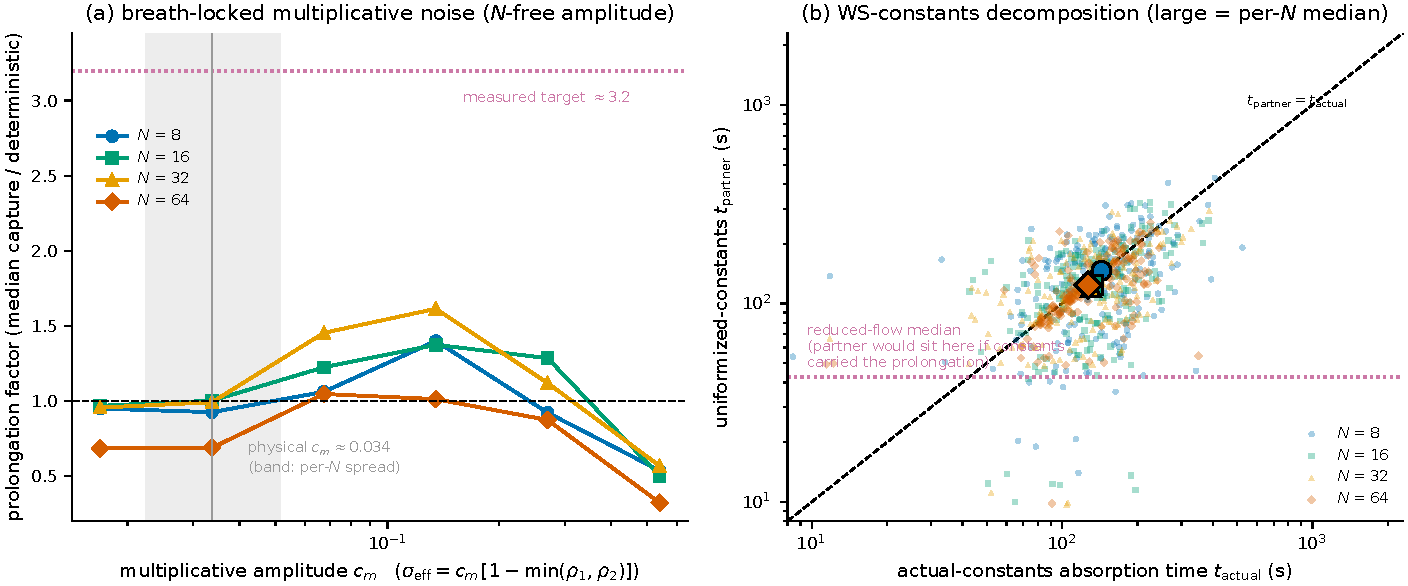
\includegraphics[width=0.95\linewidth]{fig_mech_probe}
\caption{The two remaining re-injection candidates, tested. (a)~Multiplicative
breath-locked noise $\sigma_{\mathrm{eff}} = c_m [1-\min(\rho_1,\rho_2)]$
($N$-free amplitude by construction): prolongation factor versus $c_m$ at
$A = 0.5$, $\beta = 0.05$. At the physical amplitude (vertical line; band =
per-$N$ spread of the measured estimate) the factor is $\approx 1$, and no
amplitude raises it beyond $1.4$ --- envelope-gated noise cannot re-inject from
the capture region, and at large $c_m$ it accelerates capture. (b)~Constants
decomposition: absorption time of the constants-uniformized partner versus the
actual seed ($200$ seeds per $N$; large symbols are per-$N$ medians). The pairs
sit on the diagonal, a factor $\approx 3$ above the reduced-flow median
(dotted): uniformizing the Watanabe--Strogatz constants does not remove the
prolongation.}
\label{fig:mechprobe}
\end{figure}

\section{Generality of the post-homoclinic regime across the $(\beta, A)$ plane}\label{app:corner}

Section~\ref{sec:reduced} and Appendix~\ref{app:beta} establish the
post-homoclinic inversion at two phase lags. This appendix asks, within the
reduced model, whether the inversion --- and the aging shape of the collapse-time
distribution --- is a property of those corners or of the post-homoclinic region
as a whole. We traced the homoclinic curve $A_{hc}(\beta)$ at $35$ values of
$\beta \in [0.03, 0.20]$ by the escape-to-sync bisection of
Sec.~\ref{sec:reduced} (bracket width $\le 7\times10^{-5}$ everywhere;
$A_{hc}(0.05) = 0.4096$ reproduced exactly), combined it with the saddle-node
and Hopf series (Eqs.~17--18 of Ref.~\cite{abrams2008}; numeric locators agree
to $1.4\times10^{-3}$ and $8.7\times10^{-4}$), and classified a $40\times40$
grid over $(\beta, A) \in [0.03, 0.20] \times [0.02, 0.55]$ into the four
regimes of Fig.~\ref{fig:diagram} (Fig.~\ref{fig:cornermap}).

The inversion is generic. At every one of the $592$ grid points above the
homoclinic curve the stationary-chimera fixed point of Eqs.~(13)--(14) persists
and is an unstable spiral: $\sigma = \mathrm{Re}\,\lambda > 0$ at all $592$
points, with $\sigma = 0.0046$--$0.0578$\,s$^{-1}$ and
$\omega = 0.14$--$0.35$\,s$^{-1}$, $\sigma$ growing with $\beta$ and with depth
beyond the homoclinic (Fig.~\ref{fig:cornermap}); the operating corner
reproduces the Sec.~\ref{sec:reduced} values
($\sigma = +0.01243$\,s$^{-1}$, $\omega = 0.3277$\,s$^{-1}$). Sync is globally
attracting in practice as well as in the portrait: every ensemble run below
captured (zero censoring in $9{,}600$ integrations), as did single
canonical-seed trajectories at three additional spot points.

The aging shape is \emph{not} uniform over this region. We selected eight
post-homoclinic points spanning the wedge --- four shallow points at fixed depth
$A - A_{hc} \approx +0.020$ with $\beta = 0.03$--$0.18$, and four deep points at
$A = 0.5$ with $\beta = 0.03$--$0.16$, including the operating corner --- and at
each integrated the full Sec.~\ref{sec:reduced} canonical-seed ensemble (the
$1{,}200$ seed-mapped collective initial conditions at $N = 8$--$64$, $200$ per
size) through the three-variable flow to capture, $t_{\max} = 2000$\,s. (The
$200$ $N = 4$ rows are excluded: ten of them start beyond the capture threshold
--- the two-oscillator ``population'' makes the seed map degenerate, producing
$t = 0$ events on which the Weibull likelihood is undefined; including them via
a clamped fit moves the corner value from $\hat k = 1.40$ to $1.22$ and changes
no verdict.) The censored-Weibull shape was fitted with the
profile-likelihood MLE of Sec.~\ref{sec:stats} and, independently, with a
Nelder--Mead MLE with $1{,}000$-resample bootstrap intervals; the two point
estimates agree to better than $10^{-5}$ at every point
(Table~\ref{tab:cornerk}).

Aging survives everywhere at the operating corner's depth, and fails in a
narrow band along the homoclinic. All four deep points give
$\hat k = 1.30$--$1.51$ with both intervals excluding one, as does the shallow
point at $\beta = 0.18$ ($\hat k = 1.33$), where the breathing band has
narrowed on the approach to the Takens--Bogdanov point. The three shallow
points at $\beta \le 0.10$, by contrast, are statistically memoryless:
$\hat k = 0.97$--$1.02$ with confidence intervals straddling one (at
$(\beta, A) = (0.05, 0.43)$ the bootstrap interval $[0.94, 1.00]$ sits
marginally below). The capture-time quartiles show why: near the homoclinic
they are strongly right-skewed ($9.8/13.5/70.4$\,s at $(0.05, 0.43)$ versus
$37.5/62.5/85.7$\,s at the corner) --- a seed either exits promptly or is
carried around long ghost-cycle passages near the saddle, and the heavy tail
flattens the hazard. Two cautions bound the reading. First, these $\hat k$
measure the deterministic reduced flow's dispersal of the seed ensemble, not
the finite-$N$ hazard: at the operating corner itself the reduced ensemble
gives $\hat k = 1.40$ against the measured $k_{\mathrm{abs}} = 2.27$--$3.03$
(Sec.~\ref{sec:stats}), so the reduced value is a shape test, not a magnitude
prediction. Second, and consequently, the rising hazard reported in the body
is a property of the operating corner's depth beyond the homoclinic --- it
holds at that depth for every $\beta$ tested --- but it is not a property of
post-homoclinicity per se: within ${\approx}0.02$ of the homoclinic at
$\beta \le 0.10$ the reduced collapse-time distribution loses its aging shape.
This sharpens, in the same direction, the depth caveat of
Appendix~\ref{app:beta}.

\begin{table}[t]
\centering
\caption{Censored-Weibull shape $\hat k$ of the reduced-flow capture times at
the eight aging test points ($n = 1200$ canonical-seed initial conditions per
point, zero censoring at $t_{\max} = 2000$\,s). Depth is $A - A_{hc}(\beta)$;
$\sigma$ is the unstable-spiral rate at the chimera fixed point. Profile CI:
profile-likelihood $95\%$ interval (Sec.~\ref{sec:stats} fitter); bootstrap CI:
$1{,}000$-resample percentile interval (independent fitter). Bold rows have
both intervals above one.}
\label{tab:cornerk}
\begin{tabular}{llcccc}
\toprule
$\beta$ & $A$ & depth & $\sigma$ (s$^{-1}$) & $\hat k$ [profile CI] & bootstrap CI \\
\midrule
$0.03$ & $0.461$ & $+0.021$ & $0.0048$ & $1.02$ [$0.98, 1.07$] & [$0.98, 1.07$] \\
$\mathbf{0.03}$ & $\mathbf{0.500}$ & $+0.060$ & $0.0053$ & $\mathbf{1.30}$ [$1.24, 1.36$] & [$1.24, 1.37$] \\
$0.05$ & $0.430$ & $+0.020$ & $0.0093$ & $0.97$ [$0.93, 1.01$] & [$0.94, 1.00$] \\
$\mathbf{0.05}$ & $\mathbf{0.500}$ & $+0.090$ & $0.0124$ & $\mathbf{1.40}$ [$1.33, 1.46$] & [$1.33, 1.47$] \\
$0.10$ & $0.374$ & $+0.020$ & $0.0126$ & $1.02$ [$0.98, 1.06$] & [$0.98, 1.08$] \\
$\mathbf{0.10}$ & $\mathbf{0.500}$ & $+0.146$ & $0.0250$ & $\mathbf{1.51}$ [$1.45, 1.58$] & [$1.45, 1.59$] \\
$\mathbf{0.16}$ & $\mathbf{0.500}$ & $+0.179$ & $0.0398$ & $\mathbf{1.43}$ [$1.37, 1.49$] & [$1.39, 1.48$] \\
$\mathbf{0.18}$ & $\mathbf{0.339}$ & $+0.020$ & $0.0117$ & $\mathbf{1.33}$ [$1.29, 1.37$] & [$1.22, 1.53$] \\
\bottomrule
\end{tabular}
\end{table}

\begin{figure}[t]
\centering
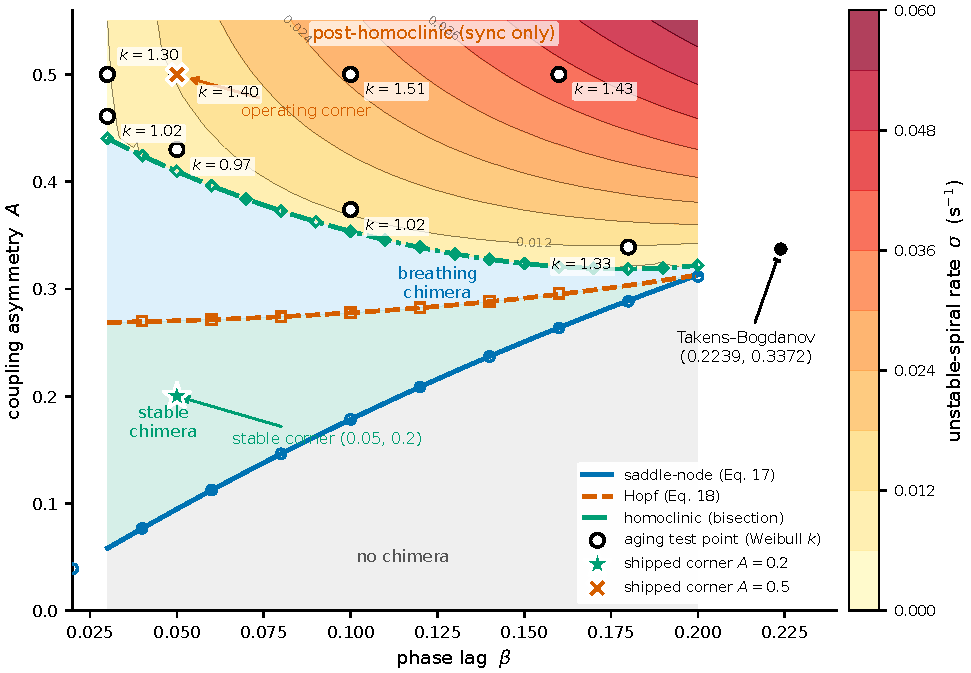
\includegraphics[width=0.95\linewidth]{fig_corner_map}
\caption{Corner-generality map. The four regimes of the $(\beta, A)$ plane
bounded by the saddle-node (Eq.~17), Hopf (Eq.~18) and homoclinic curves (the
latter traced at $35$ values of $\beta$, bisection bracket
$\le 7\times10^{-5}$), meeting at the Takens--Bogdanov point
$(0.2239, 0.3372)$. The post-homoclinic wedge is shaded by the unstable-spiral
rate $\sigma(\beta, A)$ of the persisting chimera fixed point ($\sigma > 0$ at
all $592$ grid points; labelled contours in s$^{-1}$). Open circles: the eight
aging test points with their fitted censored-Weibull shape $\hat k$
(Table~\ref{tab:cornerk}); $\hat k > 1$ at all four deep points and at the
shallow $\beta = 0.18$ point, while the shallow points at $\beta \le 0.10$
(depth ${\approx}+0.02$) are consistent with a memoryless collapse. Star and
cross: the two shipped corners.}
\label{fig:cornermap}
\end{figure}

\section{Ring hazard-shape extrapolation}\label{app:ring}

Section~\ref{sec:ring} reports that the ring's Weibull shape $\hat k$ rises with
$N$ over the campaign sizes; this appendix settles whether that rise saturates or
diverges as $N \to \infty$. The data are the per-$(\beta, N)$ censored-Weibull
shapes with profile-likelihood intervals over
$N \in \{32, 64, 128, 192, 256\}$ ($300$ runs per cell). Censoring is exactly
zero at $N \ge 64$ and at most $9.3\%$ at $N = 32$; at the extrapolation anchors
$N = 192$ and $256$ the maximum observed lifetime is
${\approx}4$--$6\times10^{3}$, far below $T_{\max} = 12{,}000$, so those fits are
entirely uncensored.

Per $\beta$, we fit $k(N)$ by least squares weighted with the per-point
uncertainty $\sigma$ (the symmetrized profile interval), comparing one bounded
form against two divergent ones: the saturating
$k(N) = k_\infty - a/N$ (two parameters), the logarithmic $k(N) = b + a \ln N$,
and the power law $k(N) = a N^{\gamma}$. Model selection is by AICc with the
small-sample penalty at $n = 5$ points (two-parameter forms cost
$\chi^2 + 10$, three-parameter forms $\chi^2 + 30$), and we call the comparison
decisive when the AICc gap between the best divergent and best saturating form
is at least $2$. Uncertainty on $k_\infty$ is bootstrapped: $5{,}000$ Gaussian
resamples of the $\hat k$ values within their $\sigma$, refit, percentile
intervals.

The saturating form wins in all five $\beta$ cells, with gaps $2.29$--$5.42$
(Table~\ref{tab:ringextrap}). Adding $N = 192$ --- the firming-up step that made
a three-parameter fit AICc-valid --- widened the three previously marginal gaps
($2.32 \to 2.98$ at $\beta = 0.110$; $2.10 \to 2.29$ at $\beta = 0.120$;
$3.87 \to 4.65$ at $\beta = 0.130$) and weakened none. The general
three-parameter form $k(N) = k_\infty - a N^{-\gamma}$ serves as confirmation
rather than selection (its third parameter costs $+20$ AICc at $n = 5$): its
$k_\infty$ agrees with the bounded fit to within $0.02$--$0.04$ everywhere, and
its $\gamma \approx 1.1$--$1.6 > 1$ says the saturation is at least as fast as
$1/N$, so the two-parameter form's fixed $\gamma = 1$ is a slightly conservative
choice. The nominally divergent fits barely diverge in any case: the fitted
logarithmic slopes are $0.05$--$0.18$ and the power exponents $0.04$--$0.13$.
All five bootstrap $k_\infty$ intervals exclude one and are tight (width
$\le 0.18$), and $k_\infty$ rises monotonically toward the existence boundary:
$1.35 < 1.49 < 1.56 < 1.62 < 1.65$ for $\beta = 0.110 \to 0.130$. The boundary
itself sits above the sweep: Appendix~\ref{app:betac} measures
$\beta_c = 0.137$ [$0.130, 0.144$], so the entire sweep approaches $\beta_c$
from below and the rise of $k_\infty$ is a rise \emph{toward} the boundary, not
across it (bootstrap probability $0.966$ that $\beta_c$ exceeds the last sweep
point $0.130$).

\begin{table}[t]
\centering
\caption{Saturate-versus-diverge model selection for the ring's $\hat k(N)$,
per $\beta$. $k_\infty$ is the bounded-fit asymptote with bootstrap $95\%$
interval; the gap is $\mathrm{AICc}(\text{best divergent}) -
\mathrm{AICc}(\text{best saturating})$, decisive at $\ge 2$; $\gamma$ is the
exponent of the confirmatory three-parameter saturating fit.}
\label{tab:ringextrap}
\begin{tabular}{lcccc}
\toprule
$\beta$ & $\hat k(N = 32 \ldots 256)$ & $k_\infty$ [$95\%$ CI] & AICc gap & $\gamma$ \\
\midrule
$0.110$ & $1.13, 1.34, 1.35, 1.38, 1.22$ & $1.35$ [$1.27, 1.43$] & $+2.98$ & $1.63$ \\
$0.115$ & $1.15, 1.52, 1.42, 1.43, 1.37$ & $1.49$ [$1.40, 1.56$] & $+5.42$ & $1.51$ \\
$0.120$ & $1.15, 1.36, 1.49, 1.46, 1.53$ & $1.56$ [$1.48, 1.65$] & $+2.29$ & $1.14$ \\
$0.125$ & $1.26, 1.64, 1.42, 1.58, 1.60$ & $1.62$ [$1.53, 1.71$] & $+2.51$ & $1.48$ \\
$0.130$ & $1.33, 1.55, 1.68, 1.68, 1.47$ & $1.65$ [$1.56, 1.74$] & $+4.65$ & $1.51$ \\
\bottomrule
\end{tabular}
\end{table}

The Sec.~\ref{sec:ring} validations carry over to the extrapolation anchors.
At $N = 256$ the dying object is a canonical chimera in $97$--$98\%$ of runs
(equilibration-gated classification of the re-run fields), and the
equilibration-filtered refits --- dropping runs in which no chimera ever
established together with the rare degenerate channel --- leave $\hat k$
unchanged or slightly larger, intervals still excluding one. The hazard shape is
criterion-robust across the spatial-homogeneity family
($\rho_{\mathrm{std}} < 0.04, 0.08, 0.10$, all with $0\%$ censoring), and the
one criterion that appears to disagree --- the mean-coherence level rule --- is
the diagnosed twisted-state censoring artifact of Sec.~\ref{sec:ring}
(Fig.~\ref{fig:ringcriterion}).

\begin{figure}[t]
\centering

\includegraphics[width=0.92\linewidth]{cp3_criterion}
\caption{Criterion-independence at $\beta = 0.130$. Left: median lifetime
decreases with $N$ under every death criterion (the near-boundary inversion is
not a detector artifact). Right: the Weibull shape $\hat k(N)$ stays above one
under the spatial-homogeneity ($\rho_{\mathrm{std}}$) criteria; the
mean-coherence rule's apparent dip below one at large $N$ is a censoring
artifact (twisted-state collapses mislabeled as censored), and the
artifact-corrected curve returns above one.}
\label{fig:ringcriterion}
\end{figure}

Two caveats bound the reading without weakening the call. First, four of the
five cells are non-monotonic in $\hat k(N)$ (in-band scatter about the plateau;
weighted $\chi^2 = 8$--$11$ on $3$ residual degrees of freedom), with only
$\beta = 0.120$ a clean leveling fit ($\chi^2 = 0.70$): $k_\infty$ should be
read as the plateau \emph{level}, ${\approx}1.35$--$1.68$, not a precisely
pinned asymptote. Second, the three-parameter fit is partially degenerate at
five points ($a$ and $\gamma$ are not separately identified), which is why the
headline rests on the parsimonious two-parameter form. What is firm is the
binary outcome and its direction: the saturating form wins in $5/5$ cells
($0/5$ divergent), and the limiting shape exceeds one in every cell --- the
increasing-hazard result survives the thermodynamic limit.

\section{An independent measurement of the ring existence boundary}
\label{app:betac}

The campaign sections take the ring chimera's existence boundary
$\beta_c \approx 0.13$--$0.14$ from the literature; this appendix turns that
citation into a measurement with the same frozen pipeline (integrator, initial
conditions, death criterion $\rho_{\mathrm{std}} < 0.04$ sustained $50$ time
units, $T_{\max} = 12{,}000$). The operational endpoint was fixed before the
ladder ran, on design probes only. Per $(\beta, N)$ cell,
$P_{\mathrm{persist}}$ is the fraction of runs that (a)~establish a chimera ---
the equilibration gate of Sec.~\ref{sec:ring}, maximum $\rho_{\mathrm{std}}$
over the live window $[50, \tau]$ exceeding $0.08$ --- and (b)~survive past a
fixed horizon $T^{*} = 400$ time units, the pooled median lifetime of the last
pre-registered cell $\beta = 0.130$ (medians $422/404/345$ at
$N = 64/128/256$), roughly twice the ${\approx}200$--$250$ decay time of the
initial-condition transient that survives above the boundary. The boundary
estimate $\beta_c(N)$ is the midpoint of a four-parameter logistic (free floor
and ceiling, binomial maximum likelihood) fit to $P_{\mathrm{persist}}(\beta)$
over the ladder $\beta = 0.115$--$0.170$ in steps of $0.0025$ ($100$ runs per
cell, $N \in \{64, 128, 256\}$, $6{,}900$ runs, zero censoring, globally unique
seeds disjoint from all prior campaigns); intervals are percentile bootstrap
over runs within cells ($B = 2{,}000$).

Establishment never fails appreciably ($\ge 95\%$ in every cell): crossing the
boundary does not prevent the seeded chimera from forming, it shortens its
life. $P_{\mathrm{persist}}$ falls from a plateau of $0.59$--$0.75$ at
$\beta \le 0.1225$ to a floor of $0.05$--$0.29$ at $\beta \ge 0.16$
(Fig.~\ref{fig:betac}a) --- the floor is nonzero because slowly decaying
traveling-wave remnants occasionally outlive $T^{*}$. The logistic midpoints
are $\beta_c(64) = 0.130$ [$0.128, 0.136$], $\beta_c(128) = 0.136$
[$0.128, 0.140$], and $\beta_c(256) = 0.134$ [$0.129, 0.141$]. Extrapolating
$\beta_c(N) = \beta_c^{\infty} + a/N$ (weighted least squares; the $1/N$ form
beats $1/\sqrt{N}$ on $\chi^2$, $0.68$ versus $0.87$ on one degree of freedom)
gives
\[
\beta_c^{\infty} = 0.137 \; [0.130, 0.144],
\]
with the $1/\sqrt{N}$ form at $0.141$ [$0.128, 0.152$] --- a form systematic of
${\approx}0.004$, smaller than the statistical interval. Moving the horizon to
$T^{*} = 300$ or $500$ moves the extrapolated midpoint to $0.142$ or $0.135$, a
comparable systematic; under every variant the boundary stays inside
$0.13$--$0.15$. The robustness endpoint --- the knee where the median lifetime
of established runs meets the post-boundary transient floor
(Fig.~\ref{fig:betac}b) --- sits higher, at $\beta = 0.155$--$0.164$ across
$N$: the persistence midpoint marks the center of the crossover, the knee its
upper edge, and together they say the boundary is a soft crossover in this
finite-$N$, fixed-criterion setting rather than a sharp threshold. As a
consistency check, the two ladder rungs shared with the main campaign
($\beta = 0.125, 0.130$; disjoint seeds, $100$ versus $300$ runs) reproduce the
published median lifetimes within sampling error.

Two readings follow. First, the measured $\beta_c^{\infty} = 0.137$
[$0.130, 0.144$] lands inside the literature range $0.13$--$0.14$ the
manuscript previously only cited. Second, the $k_\infty$ ladder of
Appendix~\ref{app:ring} ($1.35 \to 1.65$ over $\beta = 0.110 \to 0.130$) rises
toward a boundary that sits above its last rung with bootstrap probability
$0.966$ (Fig.~\ref{fig:betac}d), so ``rising monotonically toward $\beta_c$''
is geometrically coherent --- with the honest caveat that the bootstrap
interval grazes $0.130$ rather than excluding it outright, and that
$\beta_c(N)$ is measured at three sizes, so the extrapolation leans on the
form-robustness reported above.

\begin{figure}[t]
\centering
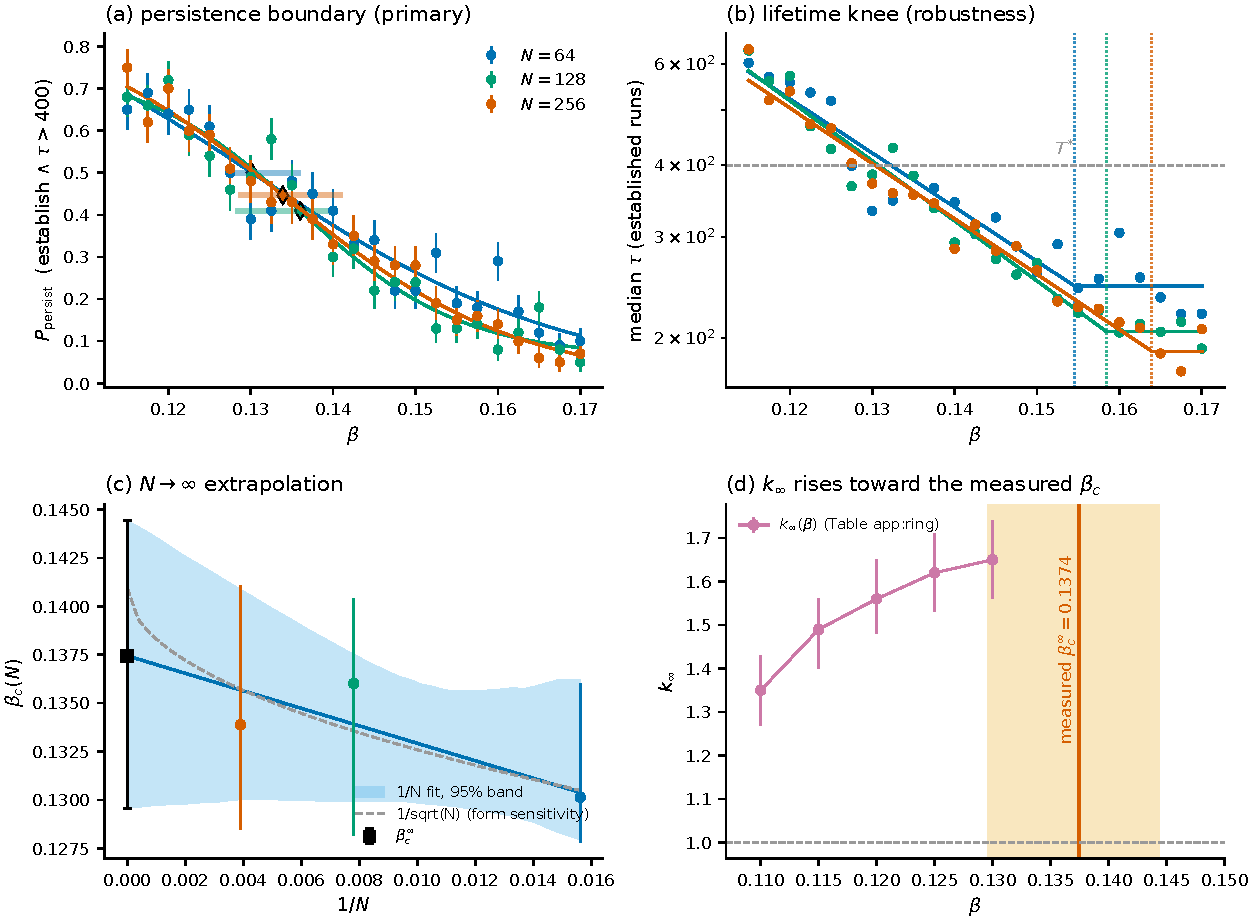
\includegraphics[width=\linewidth]{fig_betac}
\caption{Independent measurement of the ring existence boundary.
(a)~$P_{\mathrm{persist}}(\beta)$ (establish $\wedge$ $\tau > T^{*} = 400$) per
$N$ with four-parameter logistic fits; diamonds mark the midpoints
$\beta_c(N)$ with bootstrap $95\%$ intervals. (b)~Median lifetime of
established runs: a decline meeting the post-boundary transient floor at the
knee (dotted verticals), the robustness endpoint. (c)~$\beta_c(N)$ versus
$1/N$ with the bootstrap band of the $1/N$ extrapolation and the
$1/\sqrt{N}$ form for the systematic; the square is
$\beta_c^{\infty} = 0.137$ [$0.130, 0.144$]. (d)~The $k_\infty(\beta)$ ladder
of Table~\ref{tab:ringextrap} rises toward the measured boundary (vertical
line; shaded $95\%$ interval).}
\label{fig:betac}
\end{figure}

\end{appendices}

\bibliography{death_of_a_chimera_nld}

\end{document}
